\documentclass[12pt,parskip]{komatufte}
\usepackage[subpreambles=false]{standalone}

%%%%%%%%%%%%%%%%%%%%%%%%%%%
% Silence warning messages
\usepackage{silence}
\WarningsOff[scrlayer-notecolumn]
\WarningsOff[biblatex]

%%%%%%%%%%%%%%%%%%%%
% Commenting

%\usepackage[author=Lyndon]{pdfcomment}
%\newcommand{\pdfcomment}[1]{} %ignore all comments

%\usepackage{todonotes}
%\newcommand{\pdfcomment}{\todo}


%%%%%%%%%%%%%%%%%%%%
% Tables
\usepackage{booktabs}

%%%%%%%%%%%%%%%%%%%
% Fonts
\usepackage{tgadventor} %sans
\usepackage{tgpagella}  %serif
\usepackage{inconsolata} %mono
\usepackage[T1]{fontenc}

\usepackage{microtype}
\usepackage[all]{nowidow}
%%%%%%%%%%%%%%%%%%%%%%%
% Styling
\setcounter{secnumdepth}{4}
\setcounter{tocdepth}{2}

\usepackage{placeins}



%%%%%%%%%%%%%%%%%%%
% Math
\usepackage{amsmath, amssymb, stmaryrd, mathtools}
\DeclareMathOperator*{\argmin}{argmin}
\DeclareMathOperator*{\argmax}{argmax}

\usepackage{xparse,xstring,etoolbox}
% crossref this against notation section
\newcommand{\vv}[1]{\tilde{#1}} % vector
\newcommand{\seq}[1]{\mathcal{#1}} % sequence
\newcommand{\set}[1]{\mathbb{#1}} % set

%%%%%%%%%
% Indexing/sequence indexing
\newcommand{\seqind}[2]{#1^{#2}} % seqence index
\newcommand{\ind}[2]{#1_{#2}} % indexed
\newcommand{\disamb}[2]{#1^{\mathrm{#2}}} %disambiguated

%% Smart indexing and naming
\newcommand{\ifupper}[3]{
    \normalexpandarg
	\exploregroups
	\StrCount{ABCDEFGHIJKLMNOPQRSTUVWXYZ}{#1}[\uppercount]
	\ifnumgreater{\uppercount}{0}{#2}{#3}
}

%smart index
\DeclareDocumentCommand{\ii}{u{_} m}{
	\ifupper{#1}%
	{% just a single uppercase character, i.e. a matrix
		  %make sure the index is the right length
		\StrCount{#2}{,}[\indcount]
		\ifnumgreater{\indcount}{0}
		{ % Got multiple indexes so all good
		 	\ind{#1}{#2}
		}
		{ % Only 1 index so grab the column
		 	\ind{#1}{{:,#2}}
		}
	}%
	{% Not just a single upper case character
		\ind{#1}{#2}
	}
}

\DeclareDocumentCommand{\nn}{u{_} m}{
	\seqind{#1}{#2}
}

\DeclareDocumentCommand{\dd}{u{_} m}{
	\disamb{#1}{#2}
}

% Index of a vector
\DeclareDocumentCommand{\iv}{u{_} m}{\ii{\vv #1}_{#2}}
\DeclareDocumentCommand{\dv}{u{_} m}{\dd{\vv #1}_{#2}}
\DeclareDocumentCommand{\nv}{u{_} m}{\nn{\vv #1}_{#2}}

%exp
\let\oldexp\exp
\renewcommand{\exp}[1]{\oldexp \left( #1 \right)}
\newcommand{\exptwo}[1]{\oldexp_2 \left( #1 \right)}

\newcommand{\softmax}{\mathrm{smax}}

\DeclareMathOperator*{\expectedop}{\mathbb{E}}
\DeclareDocumentCommand{\expected}{u{_} m}{
	\expectedop\limits_{\mathrlap{#2}}
}

%%%%%%%%%%%%%%%%
%Graphics
\usepackage{tikz}
\usetikzlibrary{positioning, fit,  shapes.geometric}
\usepackage{ifthen}
\usepackage{etoolbox}

\tikzset{
	backgroundcolor/.style ={fill=white},
	every node/.append style={
		minimum height=7mm,
	},
	labe/.append style={
		%Blue,
		align = center,
		backgroundcolor,
		fill opacity=0.6,
		text opacity=1,
		font={\footnotesize\itshape}	
	},
	layer/.append style={
		draw,
		align = center,
		minimum height=7mm,
	},
	tight/.append style={
		inner sep=0.2mm,
	},
	lookupbox/.append style={
		draw=none,
		append after command={
		       	[shorten <= -0.5\pgflinewidth]
		       	([shift={(-1.5\pgflinewidth,-0.5\pgflinewidth)}]\tikzlastnode.north east)
		       	edge([shift={( 0.5\pgflinewidth,-0.5\pgflinewidth)}]\tikzlastnode.north west) 
		       	([shift={( 0.5\pgflinewidth,-0.5\pgflinewidth)}]\tikzlastnode.north west)
		       	edge([shift={( 0.5\pgflinewidth,-1.5\pgflinewidth)}]\tikzlastnode.south west)            
		       	([shift={( -1.5\pgflinewidth,+0.5\pgflinewidth)}]\tikzlastnode.south east)
		       	edge([shift={(-1.5\pgflinewidth,-0.5\pgflinewidth)}]\tikzlastnode.north east)
		},
		inner sep=0.7mm,
		outer sep=0mm,
		minimum width=25mm
	}
}

\usepackage{pgfplots}
\pgfplotsset{compat=1.14}
\pgfplotsset{sideplot/.append style={
		width=\notescolwidth,
		domain=-10:10,
		samples=101,
		smooth,
		enlarge y limits={abs=2},
		axis lines=middle,
		xlabel  = $z$,
		ylabel  = $y$,
	},
	equ/.append style={
		color=blue,
		thick,
		mark=none
	}
}

% Function  For a plot 
% it  needs to be declared in preamble because of how \makenote* interacts with multiple files
\def\errorsurface(#1,#2){(0.5*#1 + 0.7*#2 + sin(deg(1.5*#1 + #2^2)))^2}


\usepackage{graphicx}
\graphicspath{{./figs/}, {./}, {./figs/chaptersentencerrepr/}, {./figs/chapterintromachinelearning/}, {./figs/chapterwordrepr/}}
\usepackage{adjustbox}


%%%%%%%%%%%%%%%%%%%
% Refs
\usepackage{cleveref}

\addbibresource{master.bib}

%%%%%%%%%%%%%%%%%%%%
% Formatting

% for examples from natural language space.
\newcommand{\natlang}[1]{\ifmmode \text{``\texttt{#1}''} \else {``\texttt{#1}''}\fi}
% \ifmmode ``trick'' from https://tex.stackexchange.com/a/15194/5834

%%%%%%%%%%%%%%%%%%%%%


\begin{document}
	

\setchapterpreamble{%
	\dictum[J. M. G. ele Lammens, PhD Dissertation,
	\textit{A~Computational Model of Color Perception and Color Naming},  State University of New York, 1994]{%
Whether one sees the artificial neural network technique described below as learning or as optimization depends largely on one's background and one's theoretical likes and dislikes. I will freely use ``learning'' in the remainder of this section because that term is traditionally used in the neural networks literature, but the reader should feel free to substitute ``optimization'' if (s)he finds the other term offensive. Please contact the author for an Emacs lisp function to enforce the usage of choice.%
}}
\chapter{Introduction to neural networks for machine learning}\label{sec:machine-learning-for-representations}
\begin{abstract}
This chapter is a introduction to machine learning via neural networks.
It is 
Chapter 2: Introduction to machine learning for representations (10 pages)
This chapter can be skipped by readers already familiar with machine learning
This will not cover all aspects of machine learning, which of-course could be an entire book on its own.
It will cover the crucial basic techniques used in the works discussed in part B. The main focus will be on introducing neural networks, going into reasonable detail on hyper-parameters such as activation functions and layer sizes, as well as covering training techniques. 
It will not cover techniques that are special to natural language processing – those will be discussed in chapters 4,5, and 6.
\end{abstract}

Machine learning, particularly neural networks has become a hot topic of late.
This chapter does not serve as a complete foundational text on neural networks,
but it does cover the basics and then some as is required to understand the remainder of this book.
Readers already familiar with neural networks can skip over this chapter.


We begin with the consideration of a multivariate linear function.
We can see that this can project any point in $X$ to any point in $Y$ but that all points must move together along a straight line.

Consider instead the Logistic or sigmoid linear function:
This can project any point in $X$ to a point in $[0,1]^n$,
to a fuzzy yes-no.
But it all must move in a straight-ish line together.

\section{Function Approximation}
\aside[Multilayer perception or Artificial Neural Network?]{A artifical neural network is sometimes called a multilayer perception.
This is in reference to the related perception learning algorithm.
This term has fallen out of favor in newer works,
with Hinton, who originally coined the term, expressing his own regret at the naming.
}

The universal approximation theorem (UAT) tells us that a neural network can be used to approximate any continuous bounded function.
Here a function should be understood in the general sense -- classification is a function from observations to classes, regression is a function from observed values to target values.
More precisely it states that for a network with sufficient width
\pdfcomment{Finish this paragraph with math and citations}

A network without any hidden layers is only able to approximate linear functions.
It is equivalent to a perception, or a linear SVM. 


However, the UAT does not tell us the values for those weight parameters,
nor does it promise that any method of training will ever reach them in finite time.
More significantly it does not inform as to how wide \emph{sufficiently wide} is,
nor if deeper is more efficient than wider.


\section{Network Hyper-parameters}
\aside[Hyper-parameters vs Parameters]{
	The weights and biases of the network are called its parameters.
	They are optimised during training.
	The other features of the network, including its topology, activation functions, and the training method (which often has its own set of options), are called the hyper-parameters. 
}

The key determination in applying neural networks to any problem,
is the choice of the hyper-parameters.
Neural networks can largely be thought-off as black-boxes,
that can accomplish a, potentially poorly specified, task if given as set of examples in the form of correct outputs for given inputs.
Where the expertise in deploying a neural network solution comes in, is in the choice of the hyper-parameters of the network.

\subsection{Width and Depth}

Early neural networks often had many layers.
With the UAT showing that only one hidden layer was required then tend to become more shallow, and
with difficulties in training deeper networks.

In the last decade, deep nets have come back into fashion.
The reasons for this are out of scope for this work.
In brief it is a combination of a better techniques (e.g. RELU, unsupervised pretraining),
better hardware (e.g. GPUs and Xeon Phis), and more labeled data (e.g. from crowd-sourcing platforms such as Amazon Mechanical Turk.)

\aside[What happened to Deep Belief Network Pretraining?]{
	\textcite{hinton2006fastDBN,bengio2007greedylayerwise} lead to a new resurgence of interest in neural networks.
	Pretraining with Deep Belief Networks allowed for deep networks to be trained.
	It was held for many years that it was necessary to use layer-wise unsupervised pretraining,
	even when one has only supervised data. 
	\textcite{glorot2011deepRELUsparse} showed that with ReLU units, a deep network could be trained directly and archive the same performance.
	As such unsupervised pretraining is now a more niche technique used primarily when there is an excess of unsupervised data.
}
It has been generally found that deeper networks can have significantly few total neurons than for the same performance as wider shallower networks.

The choice of the number of hidden layers (depth),
and the sizes (width) is a key parameter in designing a neural network.
It is arguably \emph{the} key parameter.
It can be assessed using a hyper-parameter sweep on a validation or development dataset.
It is a particularly relevant parameter for our purposes, as hidden layer width forms the basis of our representations.



\subsection{Activation functions}

\aside[Notation: Generic Activation Function $\varphi$:]{Though-out this book, when the activation function is not significant to the problem at hand, we will represent it with the \mbox{symbol $\varphi$.}}
The universal approximation theorem requires that the hidden layer non-linearity be non-constant, monotonic and bounded.
In practice one does not even require that, using the unbounded RELU activation functions.
There are a wide variety of activations functions in use.
For the hidden layers these generally perform relatively similarly.
Sigmoid, tanh, and ReLU are the most common activation functions used for hidden layers.
We suggest consulting a more in-depth work on neural networks with a focus on the machine learning aspects to gain a understanding of their pros and cons.

More significantly, the final activation function or the output function does always matter.
The output function should be chosen for the task at hand.

In the following sections $y$ is the predicted final output of the network it is normally a vector, $z$ is the output from the final hidden layer again normally a vector.

\subsubsection{Linear/Affine}
A linear or affine output-layer is the most general output layer.
It is the normal output layer for use on regression or function approximation tasks.
\begin{equation}
y=Wz + b
\end{equation}
In this equation $W$ and $b$ are a trained matrix and vector respectively.
This allows the output to be any value, within some set of bounds learned during training.
However, when this is not needed it increases the difficulty of training for no benefit.
One can consider the Linear output layer as being a learned scaling and shift of the output of any of the other activation functions.
Conversely, one can look at all other activation functions as being a non-linear transformation of an linear layer, as in a traditional neural network a affine transformation is done before all other activation functions.

Linear layers, cannot on their own, be used as hidden layer activation functions.
A stack of linear layers simplifies to be equivalent to a single linear layer, which means that the network can only approximate linear functions.
A non-linearity is required.
This is what the other activation functions provide


\subsubsection{Sigmoid}
This is the classic neural network activation function.
\begin{equation}
y=\sigma{z}=\frac{1}{1+e^{-z}}
\end{equation}
Sigmoid output values are between zero and one.
If the network has a single output then this is a fuzzy boolean.
It can be used to classify into 2 categories.
It is sometimes call a logistic output.

\subsubsection{Softmax}
Softmax is the standard output layer for categorical classification.
\begin{equation}
y=s_m(z)=\left( \frac{e^{z_i}}{\sum_{j=1}^{j=N} e^{z_j}} \right)_{i=1}^{i=N}
\end{equation}
For $N$ the number of outputs equal to the number of categories attempting to be classified into.
These outputs have  values are between zero and one, and sum to one.
They are taken as a probabilistic description of the likelihood of each class.
i.e. a discrete, probability mass function (pmf).


Softmax is a \emph{soft}, i.e. differentiable,  version of what could be called \emph{hard-max}.
In this conceptual hard-max function, the largest output is set to one, and the others set to zero.
It is non-differentiable and thus not suitable for use in a neural network.
In softmax the largest values is proportionally increased to be closest to one,
and the smallest to be closest to zero.

A neural network classifier with a softmax output layer is sometimes called a multinomial logistic regression network.
This can lead to some confusion with a sigmoid outputting network.
However, the similarity can be understood by considering a softmax output layer with 2 classes.
This reduces to $s_m(z)= \left( \sigma(z), 1-\sigma(z) \right)$.


\subsubsection{Tanh}
The hyperbolic tangent function is a  scaled and shifted sigmoid function.

\begin{equation}
y=\tanh(z)=\frac{e^{2z}-1}{e^{2z}+1}=2\sigma(2z)+1
\end{equation}

The notable difference is that outputs are restricted to be between $-1$ and $+1$

\subsubsection{RELU}
The Rectified Linear Unit (ReLU) is a more recently popularized activation function \pcite{dahl2013reludropout}.
It comes from much earlier work on by neuroscience \pcite{hahnloser1998piecewise}.
\begin{equation}
y=ReLU(z)=\max \left( 0, z \right)=\begin{cases}
z & 0\le z\\
0 & z<0
\end{cases}
\end{equation}
Values are restricted to be at non-negative.
As this function has derivative zero for $z<0$, once a unit is turned off, it is not turned back-on.
Further to this, using random initialization this ensures that half of all neurons in the layer will be never turned on -- commonly called the neuron dying.
Thus resulting in sparse connections between the layers.
This has been found to be a good thing \pcite{glorot2011deepRELUsparse}.
ReLU is very commonly used as a hidden layer activation function


\subsubsection{RELU6}
\aside[Why are we bringing up ReLU6?]{ReLU6 is one of the more obsure activation functions. As such it may seem a bizare inclusion in this shorter introduction. However, we have found it surprisingly sucessful as an activation function, e.g. in the Auto-encoder example. Further to that, as a function bounded about and below it is much more theoretically nice than the ReLU unit.}

Closely related to ReLU is ReLU6.
This is another linear unit the saturates at 0, but also at 6.
\begin{equation}
y=ReLU6(z)=\max \left(0, \min\left(6, z\right) \right) =  \begin{cases}
6 & 6<z\\
z & 0\le z\le6\\
0 & z<0
\end{cases}
\end{equation}
This has similar advantages to ReLU.
however, as well as units being able to die to zero, it can also die to positive.
Unlike ReLU, it fully meets the requirements for the UAT.
The bounding at 6, rather than any other number is rather arbitrary -- particularly given scaling with the intervening affine layers.
The important point is that it is bound both above and below.




\subsubsection{Other activation functions}

There are numerous other activation functions.
Most are of interest for use in hidden layers such as Leaky RELU, Softplus, ELU and many others.
For specialized tasks, other functions might be used, such as atan2 \pcite{WhiteRepresentingAnglesSE}.




\section{Training}
The process of training the network is the process of solving a very high dimensional, nonlinear, nonconvex global optimization problem.

\aside[Evaluation function vs Loss function]{
	In this discussion we have distinguished between two types of \emph{error function}.
	The \emph{evaluation function} is the metric we are truly trying to improve, this could be accuracy for classification, BLEU score for translation, F1 score for retrieval etc. It is applied to the whole system (which may be greater than just the neural network), and the system may be evaluated in different ways using different evaluations.
	As the evaluation is often not differentiable, a proxy for it which we call the \textbf{loss function} is used in training.
	For example, squared error for regression, or cross-entropy for classification.
	The loss function is such that minimising the loss function also results in the true evaluation function being optimised.
	The loss function is applied the output of the network during training to calculate the error of a between the network output for a given input, and the target output from the example.
}

Typically, such a problem would be considered very difficult to solve.
Nonlinear and nonconvex problems can have local minima that are not global minima.
This means they can not be guaranteed to be solved  a global optima by gradient descent.
However, this does not pose an issue for more neural networks as finding the global optima is not required, merely finding a \emph{good enough} set of weights and values.

To define the training problems as an optimisation problem one first considers the loss function for a single training case.
For a target output $y$ and an actual output $\hat{y}$, a loss function is defined $loss(y, \hat{y})$.
For example the sum of squared errors loss used in regression is defined by 
$SSE(y, \hat{y})=\sum_{\forall i} (y_i-\hat{y_i})^2$.
The cross-entropy loss used in classification is defined by
$CE(y, \hat{y})=-\sum_{\forall i} (1-y_i)(\log (1-\hat{y_i}))) + y_i(\log (\hat{y_i})))$.
The choice of loss function depends on the purpose of the network.

The network function is composed into the loss function.
to the per training case loss, for a training case loss: $loss(y, N(x,\tilde{P}))$.
For $N(x,\tilde{P})$ being the function that executes some neural network, with weight and bias parameters given by $\tilde{P}$, upon an input $x$ where the target output is $y$ and the actual output is $\hat{y}$.

The total loss is defined by taking the mean over the whole train batch:
$loss_{total} = \frac{1}{K}\sum_{j=1}^{j=K} loss(y^{(j)}, N(x^{(j)},\tilde{P}))$.
This is now nothing but a nonlinear function to be minimised by adjusted the values of the weights and biases in $\tilde{P}$.
This can be given to off-the-shelf  unconstrained nonlinear optimisation algorithms \pcite{Ngiam2011} such as L-BFGS  \parencite{nocedal1980updating}.
Alternatively, and more commonly, the loss and updated can be processed iteratively on sub-sets (minibatches) of the training data at a time -- often using optimisation algorithms specifically targeted at machine learning applications.
In either case, almost all optimizers used for neural networks rely on gradient descent.

\aside[AdaGrad, AdaDelta, and Adam]{
AdaGrad \parencite(AdaGrad), AdaDelta \parencite{DBLP:journals/corr/abs-1212-5701} and Adam \parencite{kingma2014adam}
 are effectively successive iterations of an optimisation algorithm.
In all cases these algorithms dynamically adapt the learning rate during training.
There are several other algorithms in the family, both older and newer.
Adam is currently the most commonly used optimiser in recent works.
We suggest there is an interesting theoretical space about the relationship between adapting the learning rate, and implicitly finding the second derivative (the Hessian), as in the more traditional quasi-netwon methods.}


To train the network one must find the values for the networks weight and bias parameters, such that that total loss function is minimized over the training set.
$\argmin{\tilde{P}} loss_{total}(\tilde{P}, X_{train}, Y_{train})$.
As the overall loss function, including the network function, is differentiable
gradient descent can be used.
If one considers a plot with the loss given on the vertical axis,
and the values of the parameters as describing a position on the horizontal axes,
then gradient descent is moving that the parameter-point downward on that surface based on local estimate of the slope.
\pdfcomment{Insert Plot Here}
In gradient descent based methods the derivatives are calculated and then used to update the parameters.
Many advanced methods exist but the core is, for each $W \in \tilde{P}$ updating its value according to the local gradient
$W \leftarrow W - \alpha \frac{\partial loss_{total}}{\partial{W}}$, where $\alpha$ is a update step size, commonly called the learning rate.
The method of calculating the gradients: $\frac{\partial loss_{total}}{\partial{W}}$
is known as back-propagation.
Back-propagation is simply a method of applying the well-known chain-rule of calculus to the neural network loss functions \pcite{backprop}.
However, this innovation was core to allowing neural networks as we know them to be trained.





\aside[What is Backpropergation?]{%
	It is worth emphasizing that back-propagation is not a method for training neural networks.
	It is a method of applying calculus to determine the error (loss) gradient, with respect to the network parameters (weights and biases), so that gradient descent based methods can be use for optimizing those parameters.
	Some works incorrectly say ``Trained with back-propagation'', when they mean to say ``trained with gradient descent''.
}





\section{Type of Neural Network}
We will discuss more linguistically relevant neural networks in the following chapters.
However, to introduce the topic, we will give some basic examples.

\subsection{Classifier}
As one of the most basic networks, consider a classifier on the classic MNIST challenge.

\documentclass{standalone}

\usepackage{tikz}
\usetikzlibrary{positioning, fit,  shapes.geometric}
\usepackage{ifthen}
\usepackage{etoolbox}

\tikzset{
	backgroundcolor/.style ={fill=white},
	every node/.append style={
		minimum height=7mm,
	},
	labe/.append style={
		%Blue,
		align = center,
		backgroundcolor,
		fill opacity=0.6,
		text opacity=1,
		font={\footnotesize\itshape}	
	},
	layer/.append style={
		draw,
		align = center,
		minimum height=7mm,
	},
	tight/.append style={
		inner sep=0.2mm,
	},
	lookupbox/.append style={
		draw=none,
		append after command={
		       	[shorten <= -0.5\pgflinewidth]
		       	([shift={(-1.5\pgflinewidth,-0.5\pgflinewidth)}]\tikzlastnode.north east)
		       	edge([shift={( 0.5\pgflinewidth,-0.5\pgflinewidth)}]\tikzlastnode.north west) 
		       	([shift={( 0.5\pgflinewidth,-0.5\pgflinewidth)}]\tikzlastnode.north west)
		       	edge([shift={( 0.5\pgflinewidth,-1.5\pgflinewidth)}]\tikzlastnode.south west)            
		       	([shift={( -1.5\pgflinewidth,+0.5\pgflinewidth)}]\tikzlastnode.south east)
		       	edge([shift={(-1.5\pgflinewidth,-0.5\pgflinewidth)}]\tikzlastnode.north east)
		},
		inner sep=0.7mm,
		outer sep=0mm,
		minimum width=25mm
	}
}

\begin{document}

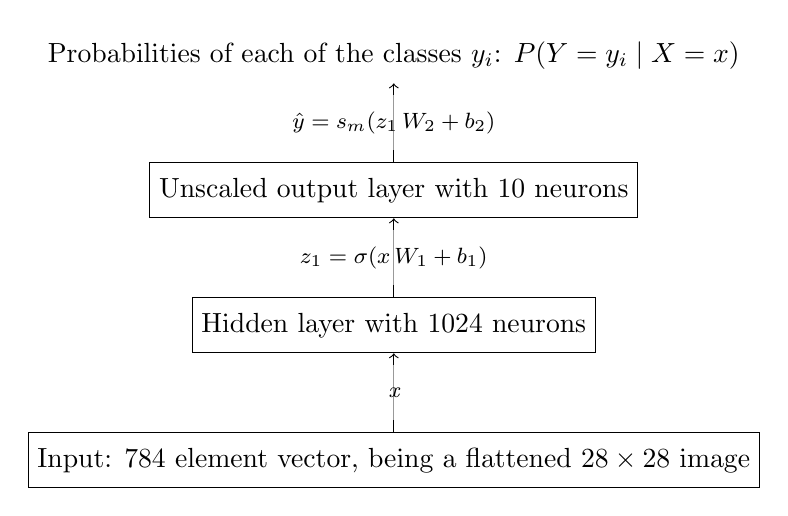
\begin{tikzpicture}[]

\node(in)[layer]{Input: 784 element vector, being a flattened $28 \times 28$ image};

\node(l1)[layer, above=of in]{Hidden layer with 1024 neurons};
\node(l2)[layer, above=of l1]{Unscaled output layer with 10 neurons};
\node(out)[above=of l2]{Probabilities of each of the classes $y_i$: $P(Y = y_i \mid X=x)$};

\draw[->] (in) edge  node[labe]{x} (l1);
\draw[->] (l1) edge  node[labe]{$z_1=\sigma(x\,W_1+b_1)$} (l2);
\draw[->] (l2) edge  node[labe]{$\hat{y}=s_m(z_1\,W_2+b_2)$} (out);

\end{tikzpicture}

\end{document}

\documentclass{standalone}

\usepackage{tikz}
\usetikzlibrary{positioning, fit,  shapes.geometric}
\usepackage{ifthen}
\usepackage{etoolbox}

\tikzset{
	backgroundcolor/.style ={fill=white},
	every node/.append style={
		minimum height=7mm,
	},
	labe/.append style={
		%Blue,
		align = center,
		backgroundcolor,
		fill opacity=0.6,
		text opacity=1,
		font={\footnotesize\itshape}	
	},
	layer/.append style={
		draw,
		align = center,
		minimum height=7mm,
	},
	tight/.append style={
		inner sep=0.2mm,
	},
	lookupbox/.append style={
		draw=none,
		append after command={
		       	[shorten <= -0.5\pgflinewidth]
		       	([shift={(-1.5\pgflinewidth,-0.5\pgflinewidth)}]\tikzlastnode.north east)
		       	edge([shift={( 0.5\pgflinewidth,-0.5\pgflinewidth)}]\tikzlastnode.north west) 
		       	([shift={( 0.5\pgflinewidth,-0.5\pgflinewidth)}]\tikzlastnode.north west)
		       	edge([shift={( 0.5\pgflinewidth,-1.5\pgflinewidth)}]\tikzlastnode.south west)            
		       	([shift={( -1.5\pgflinewidth,+0.5\pgflinewidth)}]\tikzlastnode.south east)
		       	edge([shift={(-1.5\pgflinewidth,-0.5\pgflinewidth)}]\tikzlastnode.north east)
		},
		inner sep=0.7mm,
		outer sep=0mm,
		minimum width=25mm
	}
}

\begin{document}

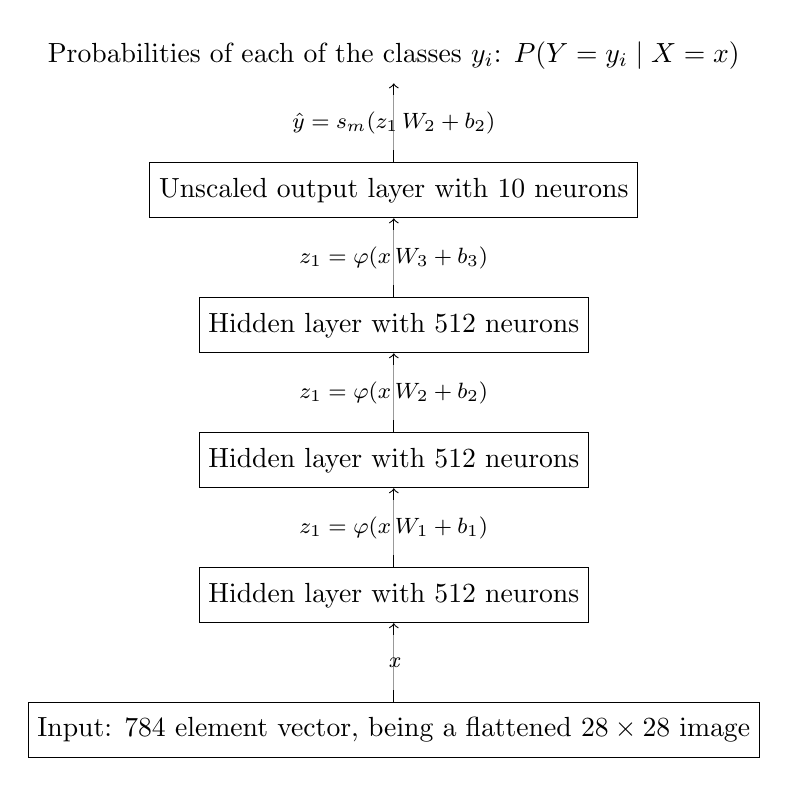
\begin{tikzpicture}[]

\node(in)[layer]{Input: 784 element vector, being a flattened $28 \times 28$ image};

\node(l1)[layer, above=of in]{Hidden layer with 512 neurons};
\node(l2)[layer, above=of l1]{Hidden layer with 512 neurons};
\node(l3)[layer, above=of l2]{Hidden layer with 512 neurons};

\node(lo)[layer, above=of l3]{Unscaled output layer with 10 neurons};
\node(out)[above=of lo]{Probabilities of each of the classes $y_i$: $P(Y = y_i \mid X=x)$};

\draw[->] (in) edge  node[labe]{x} (l1);
\draw[->] (l1) edge  node[labe]{$z_1=\varphi(x\,W_1+b_1)$} (l2);
\draw[->] (l2) edge  node[labe]{$z_1=\varphi(x\,W_2+b_2)$} (l3);
\draw[->] (l3) edge  node[labe]{$z_1=\varphi(x\,W_3+b_3)$} (lo);

\draw[->] (lo) edge  node[labe]{$\hat{y}=s_m(z_1\,W_2+b_2)$} (out);

\end{tikzpicture}

\end{document}

\subsection{Bottle Necking Auto-encoder}

\documentclass{standalone}

\usepackage{tikz}
\usetikzlibrary{positioning, fit,  shapes.geometric}
\usepackage{ifthen}
\usepackage{etoolbox}

\tikzset{
	backgroundcolor/.style ={fill=white},
	every node/.append style={
		minimum height=7mm,
	},
	labe/.append style={
		%Blue,
		align = center,
		backgroundcolor,
		fill opacity=0.6,
		text opacity=1,
		font={\footnotesize\itshape}	
	},
	layer/.append style={
		draw,
		align = center,
		minimum height=7mm,
	},
	tight/.append style={
		inner sep=0.2mm,
	},
	lookupbox/.append style={
		draw=none,
		append after command={
		       	[shorten <= -0.5\pgflinewidth]
		       	([shift={(-1.5\pgflinewidth,-0.5\pgflinewidth)}]\tikzlastnode.north east)
		       	edge([shift={( 0.5\pgflinewidth,-0.5\pgflinewidth)}]\tikzlastnode.north west) 
		       	([shift={( 0.5\pgflinewidth,-0.5\pgflinewidth)}]\tikzlastnode.north west)
		       	edge([shift={( 0.5\pgflinewidth,-1.5\pgflinewidth)}]\tikzlastnode.south west)            
		       	([shift={( -1.5\pgflinewidth,+0.5\pgflinewidth)}]\tikzlastnode.south east)
		       	edge([shift={(-1.5\pgflinewidth,-0.5\pgflinewidth)}]\tikzlastnode.north east)
		},
		inner sep=0.7mm,
		outer sep=0mm,
		minimum width=25mm
	}
}

\begin{document}

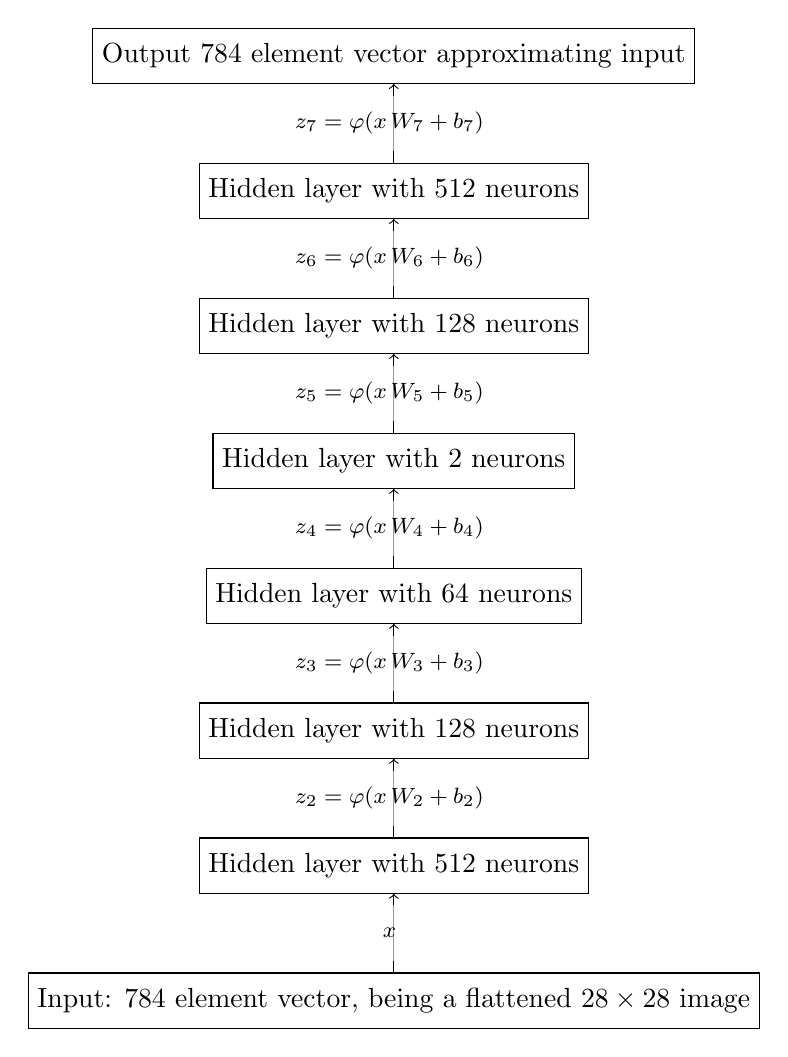
\begin{tikzpicture}[]

\node(L0)[layer]{Input: 784 element vector, being a flattened $28 \times 28$ image};

\foreach \i/\y[count=\j from 0] in {1/512, 2/128, 3/64, 4/2, 5/128, 6/512, 7/784}{
	\node(L\i)[layer, above= of L\j] {
		\ifthenelse{\j=6}{Output 784 element vector approximating input}%
		{Hidden layer with $\y$ neurons}%
	};
%
	\draw[->] (L\j) edge  node[labe]{
		\ifthenelse{\j = 0}{$x$}{$z_\i=\varphi(x\,W_\i+b_\i)$}
	}(L\i);	
}

%
\end{tikzpicture}

\end{document}

\section{Recurrent Neural Networks}
A key limitation of a neural network is that the number of inputs and outputs must be known at training time and must always be the same for all cases.
This is not true for natural language: If an over-all input is a sentence for example, then each sentence input will be made up a varying number of words.

Recurrent neural networks (RNN) over-come this by allowing the network to have a memory.
A RNN is effectively a chain of feed-forward neural networks,
each one being identical in terms of their weight and bias parameters,
but each one acting at a different time-step.





\begin{figure}
	\caption{The unrolled structure of an RNN for us in Encoding, Decoding and Encoding-Decoding (sequence-to-sequence) problems. RU is the recurrent unit -- the neural network which reoccurs at each time step.}
	
	\label{fig-rnns}

	\resizebox{\textwidth}{!}{
		\documentclass[landscape]{article}
\usepackage[a3paper]{geometry}

\usepackage{tikz}
\usetikzlibrary{positioning, fit,  shapes.geometric}
\usepackage{ifthen}
\usepackage{etoolbox}

\tikzset{
	backgroundcolor/.style ={fill=white},
	every node/.append style={
		minimum height=7mm,
	},
	labe/.append style={
		%Blue,
		align = center,
		backgroundcolor,
		fill opacity=0.6,
		text opacity=1,
		font={\footnotesize\itshape}	
	},
	layer/.append style={
		draw,
		align = center,
		minimum height=7mm,
	},
	tight/.append style={
		inner sep=0.2mm,
	},
	lookupbox/.append style={
		draw=none,
		append after command={
		       	[shorten <= -0.5\pgflinewidth]
		       	([shift={(-1.5\pgflinewidth,-0.5\pgflinewidth)}]\tikzlastnode.north east)
		       	edge([shift={( 0.5\pgflinewidth,-0.5\pgflinewidth)}]\tikzlastnode.north west) 
		       	([shift={( 0.5\pgflinewidth,-0.5\pgflinewidth)}]\tikzlastnode.north west)
		       	edge([shift={( 0.5\pgflinewidth,-1.5\pgflinewidth)}]\tikzlastnode.south west)            
		       	([shift={( -1.5\pgflinewidth,+0.5\pgflinewidth)}]\tikzlastnode.south east)
		       	edge([shift={(-1.5\pgflinewidth,-0.5\pgflinewidth)}]\tikzlastnode.north east)
		},
		inner sep=0.7mm,
		outer sep=0mm,
		minimum width=25mm
	}
}
\usepackage{amsmath, amssymb, stmaryrd, mathtools}
\DeclareMathOperator*{\argmin}{argmin}
\DeclareMathOperator*{\argmax}{argmax}

\usepackage{xparse,xstring,etoolbox}
% crossref this against notation section
\newcommand{\vv}[1]{\tilde{#1}} % vector
\newcommand{\seq}[1]{\mathcal{#1}} % sequence
\newcommand{\set}[1]{\mathbb{#1}} % set

%%%%%%%%%
% Indexing/sequence indexing
\newcommand{\seqind}[2]{#1^{#2}} % seqence index
\newcommand{\ind}[2]{#1_{#2}} % indexed
\newcommand{\disamb}[2]{#1^{\mathrm{#2}}} %disambiguated

%% Smart indexing and naming
\newcommand{\ifupper}[3]{
    \normalexpandarg
	\exploregroups
	\StrCount{ABCDEFGHIJKLMNOPQRSTUVWXYZ}{#1}[\uppercount]
	\ifnumgreater{\uppercount}{0}{#2}{#3}
}

%smart index
\DeclareDocumentCommand{\ii}{u{_} m}{
	\ifupper{#1}%
	{% just a single uppercase character, i.e. a matrix
		  %make sure the index is the right length
		\StrCount{#2}{,}[\indcount]
		\ifnumgreater{\indcount}{0}
		{ % Got multiple indexes so all good
		 	\ind{#1}{#2}
		}
		{ % Only 1 index so grab the column
		 	\ind{#1}{{:,#2}}
		}
	}%
	{% Not just a single upper case character
		\ind{#1}{#2}
	}
}

\DeclareDocumentCommand{\nn}{u{_} m}{
	\seqind{#1}{#2}
}

\DeclareDocumentCommand{\dd}{u{_} m}{
	\disamb{#1}{#2}
}

% Index of a vector
\DeclareDocumentCommand{\iv}{u{_} m}{\ii{\vv #1}_{#2}}
\DeclareDocumentCommand{\dv}{u{_} m}{\dd{\vv #1}_{#2}}
\DeclareDocumentCommand{\nv}{u{_} m}{\nn{\vv #1}_{#2}}

%exp
\let\oldexp\exp
\renewcommand{\exp}[1]{\oldexp \left( #1 \right)}
\newcommand{\exptwo}[1]{\oldexp_2 \left( #1 \right)}

\newcommand{\softmax}{\mathrm{smax}}

\DeclareMathOperator*{\expectedop}{\mathbb{E}}
\DeclareDocumentCommand{\expected}{u{_} m}{
	\expectedop\limits_{\mathrlap{#2}}
}

\begin{document}

\numdef{\N}{8}
\numdef{\labelwidth}{5.5cm}
%%%%%%%%%%%%%%%%%%%%%%%%%
% Encoder

\begin{tikzpicture}[]

\begin{scope}
	\node(lblEncoder)[text width= \labelwidth] {\textbf{RNN Encoder:}\\%
	Variable $n$ inputs: $\nv x_t$\\%
	1 output: $\hat{y}$ \\%
	};
	
	\coordinate (L0) at (lblEncoder.east);
	
	\foreach \I[count=\j from 0] in {1,...,\N}{
		\ifnumequal{\I}{\N - 1}{%
			\node(L\I)[dashed, layer, right = of L\j] {...};
			\node(w\I)[below = of L\I]{...};
		}%
		{	
			\node(L\I)[layer, right = of L\j] {RU};
			\node(w\I)[below = of L\I]{\ifnumequal{\I}{\N}{$\nv x_n$}{$\nv x_\I$}};
			\draw[->](w\I) -- (L\I);
		}
	}
	\foreach \I[count=\j from 1] in {2,...,\N} {
		\draw[->] (L\j) edge node[labe]{state} (L\I);
	}
	
	\node(out) [above = of L\N]{$\hat{y}$};
	\draw[->] (L\N) -- (out);
\end{scope}

%%%%%%%%%%%%%%%%
% Decoder
\begin{scope}[yshift=-5cm] 
\node(lbl)[text width= \labelwidth] {\textbf{RNN Decoder:}\\%
1 input: $x$\\%
variable $m$ outputs: $\n \hat{y}_t$ \\%
with prompts: $\nv r_t$ (often $\nv y_{t-1}$)
};

\coordinate (L0) at (lbl.east);
\coordinate (L1c)[right = of L0];
\node(x)[below right = 4 of L1c]{$x$};

\foreach \I[count=\j from 0] in {1,...,\N}{
	\ifnumequal{\I}{\N - 1}{%
		\node(L\I)[dashed, layer, right = of L\j] {...};
		\node(w\I)[above = of L\I]{...};
		\node(y\I)[below = of L\I]{...};
	}%
	{	
		\node(L\I)[layer, right = of L\j] {RU};
		\node(v\I)[above = of L\I]{\ifnumequal{\I}{\N}{$\n \hat{y}_m$}{$\n \hat{y}_\I$}};
		\node(w\I)[below = of L\I]{$[\nv r_\I; \v x]$};
		\draw[->](w\I) -- (L\I);
		\draw[->](L\I) -- (v\I);
		\draw[->](x) to[bend right = 5] (w\I.300);
	}
}
\foreach \I[count=\j from 1] in {2,...,\N} {
	\draw[->] (L\j) edge node[labe]{state} (L\I);
}

\end{scope}
%
%%%%%%%%%%%%%%%%%%
% Encoder Decoder
%
\begin{scope}[yshift=-14cm]
\node(lbl)[text width= \labelwidth] {\textbf{RNN Encoder-Decoder:}\\%
Variable $n$ inputs: $\nv x_t$\\%
Variable $m$ outputs $\n \hat{y}_t$\\%
Prompts: $\nv r_t$ (often $y_{t-1}$)
};

\coordinate (L0) at (lbl.east);
\numdef{\NN}{4}
\foreach \I[count=\j from 0] in {1,...,\NN}{
	\ifnumequal{\I}{\NN - 1}{%
		\node(L\I)[dashed, layer, right = of L\j] {...};
		\node(w\I)[below = of L\I]{...};
	}%
	{
		\node(L\I)[layer, right = of L\j] {$\mathrm{RU_E}$};
		\node(w\I)[below = of L\I]{\ifnumequal{\I}{\NN}{$\nv x_n$}{$\nv x_\I$}};
		\draw[->] (w\I) -- (L\I);
	}
}
\foreach \I[count=\j from 1] in {2,...,\NN} {
	\draw[->] (L\j) edge node[labe] {state} (L\I);
}




\coordinate[above = 3 of L\NN] (Lp\NN);
\numdef{\NP}{\N - 1}
\foreach \j in {\NN,...,\NP}{
	\numdef{\I}{\j+1}
	\numdef{\y}{\I - \NN}
	\ifnumequal{\I}{\N-1}{%
		\node(Lp\I)[dashed, layer, right = of Lp\j] {...};
		\node(w\I)[below = of Lp\I]{...};
		\node(y\I)[above = of Lp\I]{...};
	}%
	{
		\node(Lp\I)[layer, right = of Lp\j] {$\mathrm{RU_D}$};
		\ifnumequal{\I}{\N}{
			\node(w\I)[below = of Lp\I]{$[\v z; \nv r_m]$};
			\node(y\I)[above = of Lp\I]{$\n \hat{y}_m$};
		}
		{
			\node(w\I)[below = of Lp\I]{$[\v z; \nv r_\y]$};
			\node(y\I)[above = of Lp\I]{$\n \hat{y}_\y$};
		}

		\draw[->] (w\I) -- (Lp\I);
		\draw[->] (Lp\I) -- (y\I);
		\path[->] (L\NN.north) edge node[labe]{$\v z$} (w\I.south west);
	}
}


\numdef{\NNp1}{\NN + 1}
\foreach \I in {\NNp1,...,\NP} {
	\numdef{\j}{\I+1}
	\draw[->] (Lp\I) edge node[labe] {state} (Lp\j);
}
 

\end{scope}


\end{tikzpicture}




\end{document}
	}


\end{figure}

Three general examples of the structure of RNNs are shown in \Cref{fig-rnns}.
These exampled will be considered in more later in this section below.
At each time-step the same network is used, with different inputs.
For purposes of looking at this in the big picture we will first consider this a black-box recurrent unit (RU).




\documentclass{standalone}

\usepackage{tikz}
\usetikzlibrary{positioning, fit,  shapes.geometric}
\usepackage{ifthen}
\usepackage{etoolbox}

\tikzset{
	backgroundcolor/.style ={fill=white},
	every node/.append style={
		minimum height=7mm,
	},
	labe/.append style={
		%Blue,
		align = center,
		backgroundcolor,
		fill opacity=0.6,
		text opacity=1,
		font={\footnotesize\itshape}	
	},
	layer/.append style={
		draw,
		align = center,
		minimum height=7mm,
	},
	tight/.append style={
		inner sep=0.2mm,
	},
	lookupbox/.append style={
		draw=none,
		append after command={
		       	[shorten <= -0.5\pgflinewidth]
		       	([shift={(-1.5\pgflinewidth,-0.5\pgflinewidth)}]\tikzlastnode.north east)
		       	edge([shift={( 0.5\pgflinewidth,-0.5\pgflinewidth)}]\tikzlastnode.north west) 
		       	([shift={( 0.5\pgflinewidth,-0.5\pgflinewidth)}]\tikzlastnode.north west)
		       	edge([shift={( 0.5\pgflinewidth,-1.5\pgflinewidth)}]\tikzlastnode.south west)            
		       	([shift={( -1.5\pgflinewidth,+0.5\pgflinewidth)}]\tikzlastnode.south east)
		       	edge([shift={(-1.5\pgflinewidth,-0.5\pgflinewidth)}]\tikzlastnode.north east)
		},
		inner sep=0.7mm,
		outer sep=0mm,
		minimum width=25mm
	}
}

\begin{document}

\numdef{\n}{8}
%%%%%%%%%%%%%%%%%%%%%%%%%
% Encoder

\begin{tikzpicture}[]

\node(ru)[layer]{RU};

\node(stm)[left = of ru]{old state};
\draw[->] (stm) edge node[labe] {$s_{t-1}$} (ru);

\node(stp)[right = of ru]{new state};
\draw[->] (ru) edge node[labe] {$s_{t}$} (stp);


\node(out)[above = of ru]{output};
\draw[->] (ru) edge node[labe] {$\hat{y}_t$} (out);


\node(in)[below = of ru]{input};
\draw[->] (in) edge node[labe] {$x_t$} (ru);


\end{tikzpicture}

\end{document}




 

\end{document}